\begin{frame}{Parallelism in MLMC}
\centering
\begin{tikzpicture}[
  node distance = 1cm, 
  block/.style = {
    draw, rectangle, thick,
    minimum width=2cm, minimum height=1.0cm, 
    align=center,
    font=\footnotesize
  }
]

\node[block] (levels) {Parallelism across \\ Levels};
\node[block, right = of levels] (samples) {\textbf{Parallelism across} \\ \textbf{Samples}};
\node[block, right = of samples] (schemes) {Parallelism within \\ Schemes};

\draw[-, thick] (levels.east) -- (samples.west);
\draw[-, thick] (samples.east) -- (schemes.west);

\node[black, above=0.06cm of samples] {\scalebox{1.2}{$\downarrow$}};

\end{tikzpicture}

\begin{columns}[T] % The [T] option top-aligns the columns

    \begin{column}{0.6\textwidth}
        \vspace{3.6em}
        \begin{itemize}
            \item Parallelised MLMC algorithm over samples using OpenMP.
            \item Resulted in baseline average $\times 4$ speed improvement.
        \end{itemize}
    \end{column}

    % --- Right Column for the Graphic ---
    \begin{column}{0.4\textwidth}
        % The \centering command is optional but good practice
        \centering
        % \linewidth makes the image fit the column width
        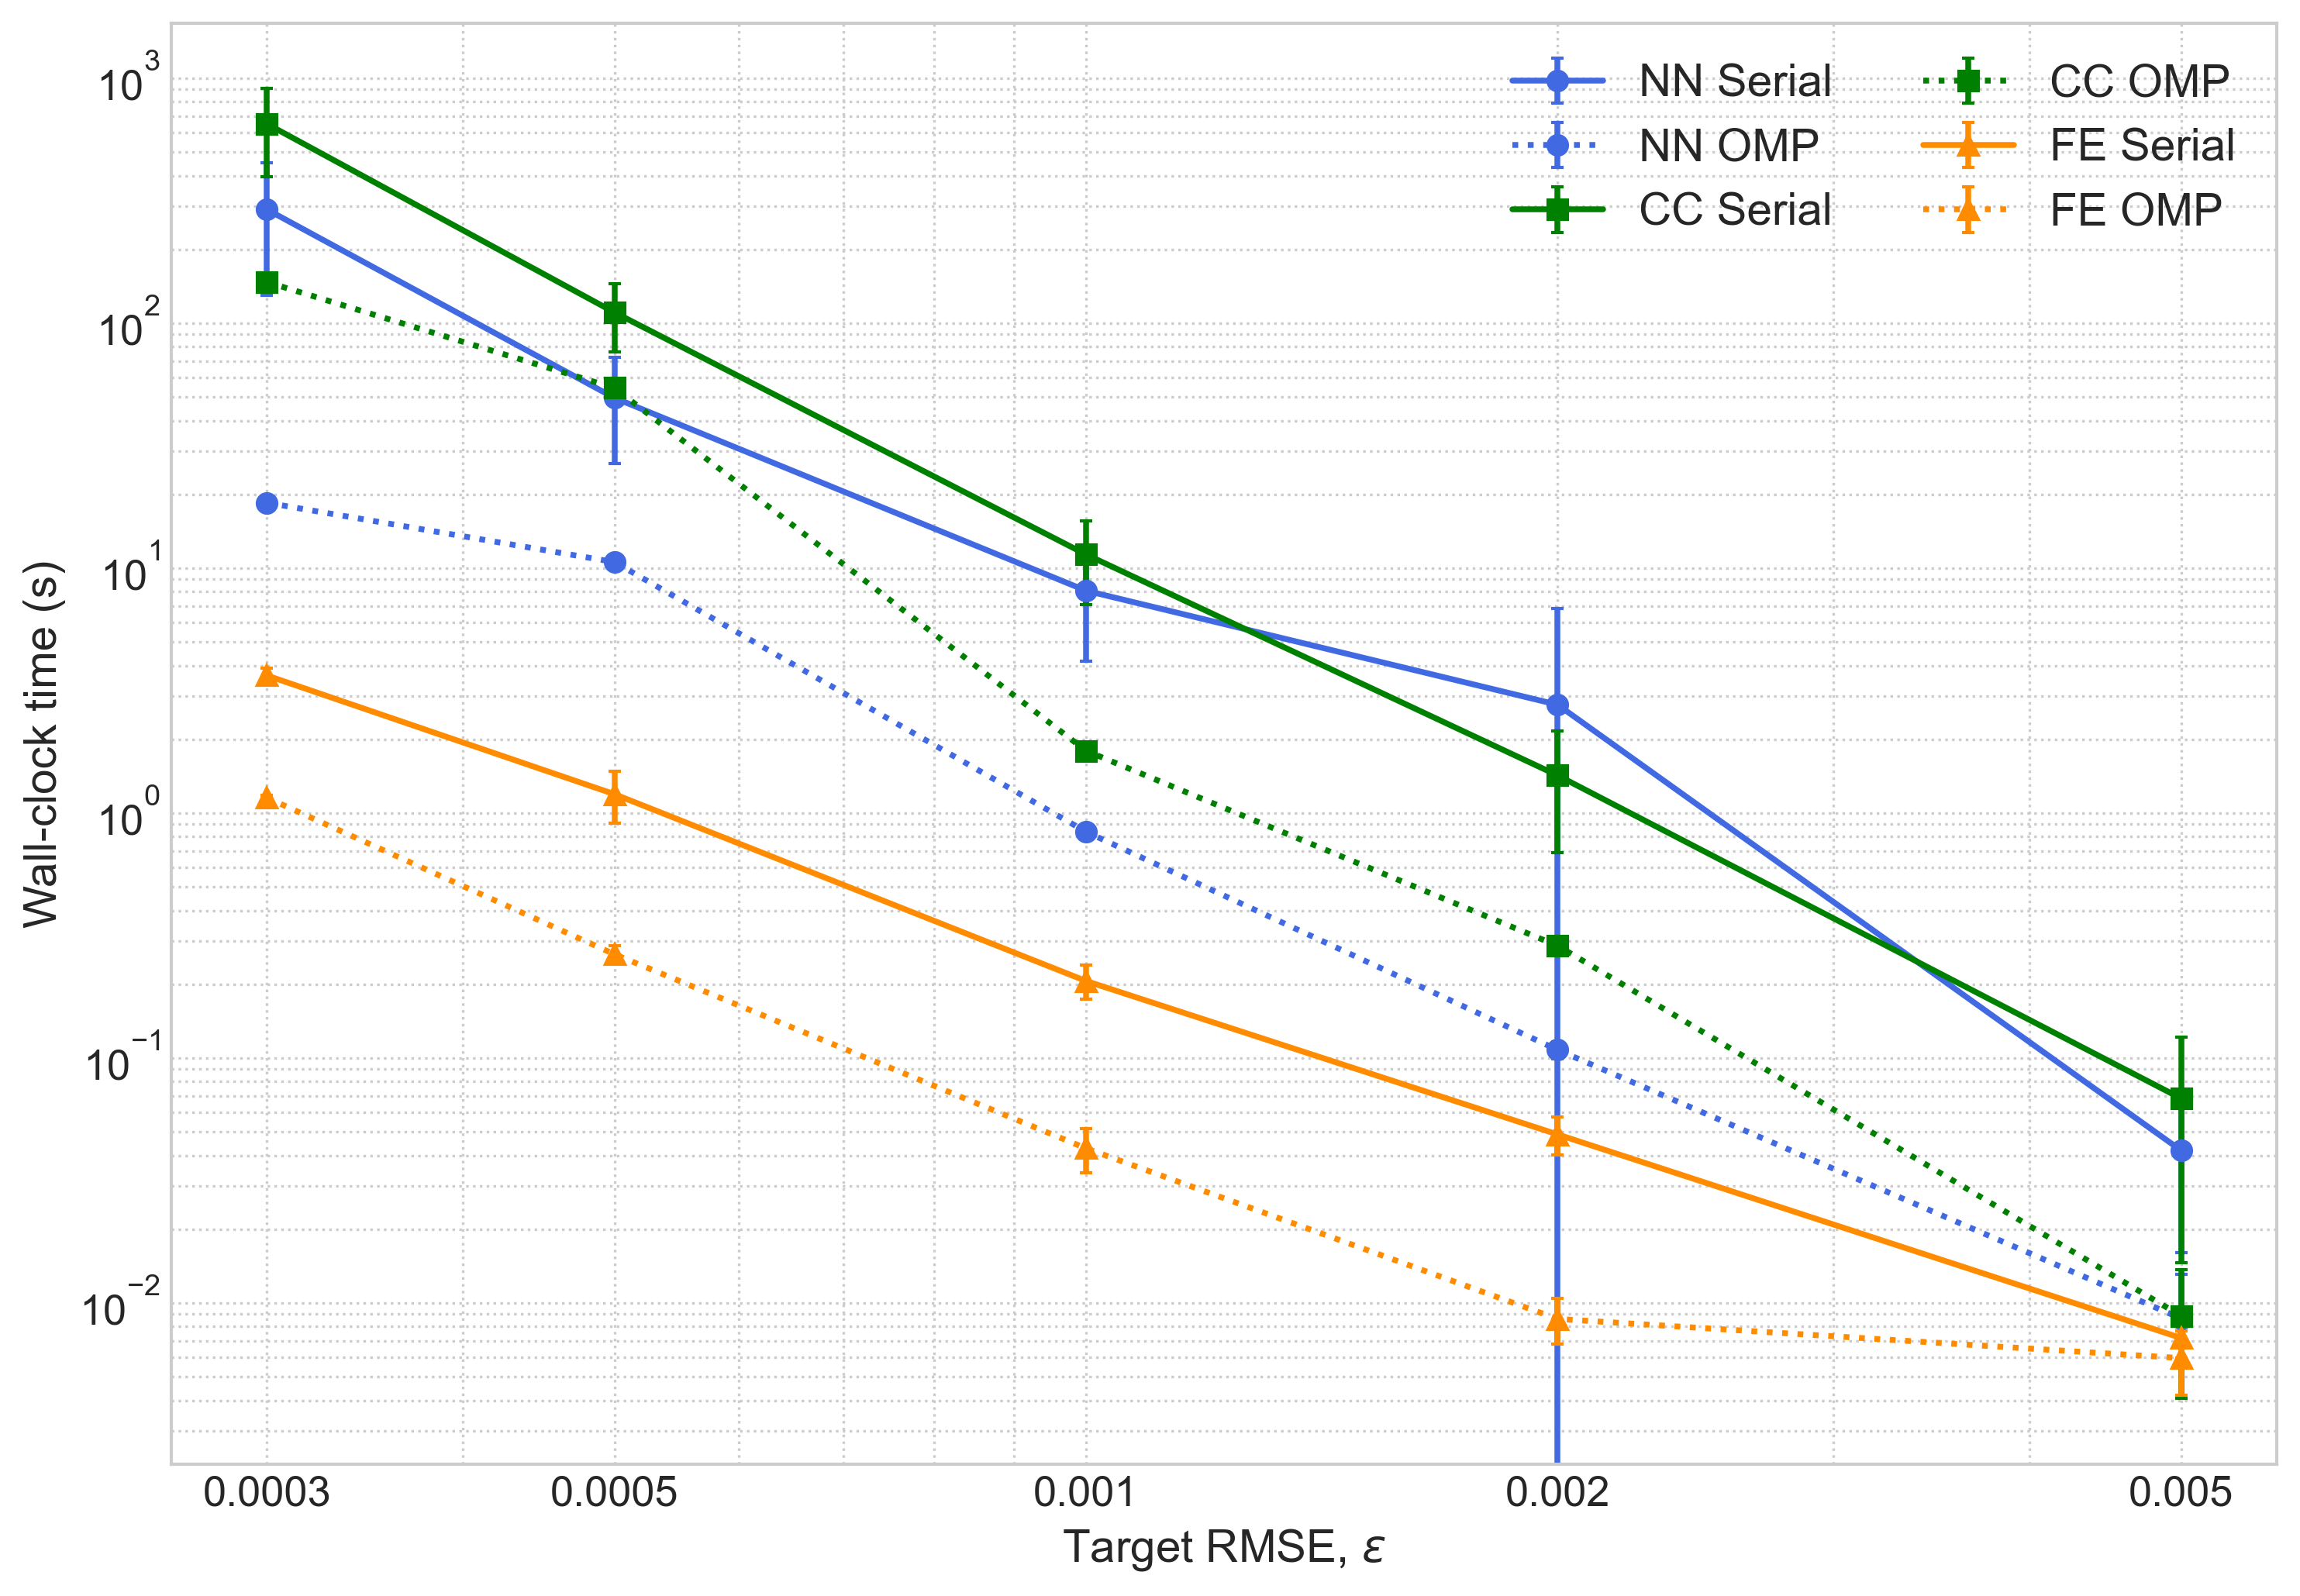
\includegraphics[width=\linewidth]{presentation_graphics/perf_wallclock_vs_eps.png}
    \end{column}

\end{columns}
\end{frame}

\begin{frame}{}
\centering
\quad Thank you for listening.
\newline

\qquad Questions?

\end{frame}

